% ============================================================================
\section{Introduction}
\label{sec:intro}
% ============================================================================
\PARstart{I}{ndonesian} employers withhold Income Tax Article 21 (PPh 21) from the pay of every employee each month, so an error in the rules reaches every payslip and every withholding slip. The rules change often. Between 2023 and 2026, 13 regulatory events changed the PPh 21 computation for permanent employees, and seven of them were issued in 2025 (Fig.~\ref{fig:timeline}). Government Regulation (PP) 58/2023 and its implementing Minister of Finance Regulation (PMK) 168/2023 replaced the annualized monthly method with average effective rates (TER) from January 2024. Both were issued in the last week of December 2023~\cite{pp58_2023,pmk168_2023}. Five events took effect retroactively. PMK 10/2025 made the government bear the tax of certain employees (DTP). It was issued on 4 February 2025 but covers January 2025, so a January payroll that was correct when it ran became wrong a month later~\cite{pmk10_2025}.

\begin{figure*}[!t]
\centering
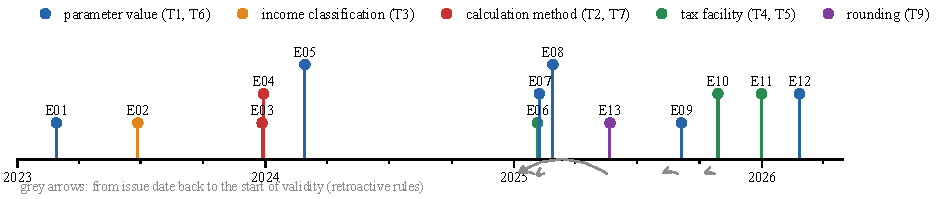
\includegraphics[width=\textwidth]{figs/fig_timeline.pdf}
\caption{Regulatory events that changed PPh 21 for permanent employees, 2023--2026, at their issue dates. Colors group the change types of Table~\ref{tab:types}; grey arrows run from the issue date back to the start of validity for the five retroactive rules.}
\label{fig:timeline}
\end{figure*}

Payroll software usually encodes these rules in program code or spreadsheets~\cite{ramadhani2021grossup,kusuma2026pph21}, so every regulation needs new code. Two open-source PPh 21 calculators added TER 26 and 915 days after PP 58/2023 was issued and changed 163 and 504 lines of code (Section~\ref{sec:res-compare}). Nothing in either change shows that earlier periods keep their results, and a company policy that the new rule makes noncompliant goes unnoticed. A knowledge-based system (KBS) separates the rules from the code that executes them~\cite{merigoux2021catala}, but the burden moves to keeping the knowledge base (KB) current. Large language models (LLMs) can turn legal text into structured rules~\cite{janatian2023texttostructure}, yet they are unreliable when asked to compute tax directly~\cite{nay2024taxattorneys,dahl2024legalfictions}.

Work that combines LLMs with tax rules builds a rule base for the law at one point in time. The closest exception updated a tax program by one legal year with LLM-written candidates selected by majority vote~\cite{goganikhiabani2025maintaining}, without testing earlier periods or a chain of updates. Earlier work has not measured whether repeated LLM-drafted updates of an executable legal rule base keep the results of earlier periods, or whether an error in one update spreads to later ones. It has also not measured how such an update affects the policies that companies layer on top of the regulation (Table~\ref{tab:position} in Section~\ref{sec:related}).

This paper addresses those questions with a KBS for PPh 21 whose knowledge is a two-layer knowledge graph, with one layer for regulations and one for company policies (Fig.~\ref{fig:architecture}). Every element of the graph records both its legal validity and the date it became known. A deterministic engine computes the tax and traces each value to the provisions it rests on. An LLM only drafts knowledge updates. Each draft must quote the document, passes five verification gates, and competes with independent drafts in a behavioral consensus that abstains when the drafts disagree; a reviewer approves the result. The study measures four properties of this design: the expressiveness of the representation, the safety of a single LLM-drafted update, the stability of updates applied in chronological order, and the detection of company policies affected by a regulatory change.

The contributions are:
\begin{enumerate}
\item A bitemporal two-layer representation of PPh 21 as an RDF knowledge graph with executable rules, conflict resolution between the layers, and a trace to the provisions (Section~\ref{sec:system}). It expressed 16 changes unseen by its designers without engine modifications once the rounding convention of their examples was aligned.
\item An incremental acquisition pipeline in which an LLM drafts updates with quoted sources, deterministic gates and behavioral consensus filter them, and a reviewer receives an impact report (Section~\ref{sec:system}). Ablations attribute its gain over a single draft to consensus and abstention, not to the gates.
\item A regulation-replay protocol that applies real changes in chronological order, in isolation and in a chain, and separates inherited, new, and triggered errors (Sections~\ref{sec:formulation} and~\ref{sec:design}).
\item An evaluation on the 13 regulatory events of 2023--2026 and five collective labor agreements that shows for which kinds of change an LLM-drafted update can be trusted (Section~\ref{sec:results}). The knowledge base, corpus, test cases, and logs are released.
\end{enumerate}
Section~\ref{sec:background} summarizes PPh 21 for readers outside Indonesia, Section~\ref{sec:related} positions the work, Sections~\ref{sec:formulation}--\ref{sec:casestudy} define the problem and the system, Sections~\ref{sec:design}--\ref{sec:results} report the evaluation, and Sections~\ref{sec:discussion} and~\ref{sec:conclusion} discuss and conclude.
